\section{Autonomous Walking}
\label{sec::52_aw}
The autonomous walking is based upon the performance within the test environment from section \ref{sec::512_pt}. The found parameters are used for comparative reason throughout this section as well. As explained in section \ref{sec::324_ip}, the neural network benefits strongly from an available depth map as input. We will therefore deal with the depth map extraction first.
\subsection{Camera Calibration}
As described in section \ref{sec::324_ip}, in order for the stereo block matching algorithm to work properly (equation \ref{eq::324_sad}), it is required to calibrate the cameras. We shortly verified this in figure \ref{fig::521_no_calib}, where we extracted a depth map from the uncalibrated stereo camera pair.
\begin{figure}[h]
	\centering
	\subcaptionbox{Left disparity map.}%
	[.4\linewidth]{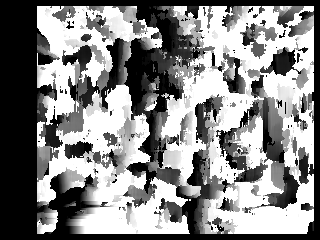
\includegraphics[scale=.3]{chapters/05_experiments/02_autonomous_walking/02_depth_map_parameter_tuning/disp_no_calib.png}}
	\subcaptionbox{Confidence weighted least squares filtered disparity map.}%
	[.4\linewidth]{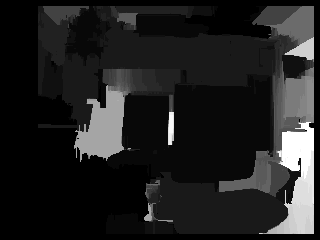
\includegraphics[scale=.3]{chapters/05_experiments/02_autonomous_walking/02_depth_map_parameter_tuning/wls_no_calib.png}}
	\caption{Depth map extraction without calibration. The parameters were set as follows to $N=13$, $D=32$, $\sigma = 1$, and $\lambda=10^4$.}
	\label{fig::521_no_calib}
\end{figure}
For the calibration we chose to use a chess-board calibration pattern, see figure \ref{fig::521_calib}. The used calibration pattern has width of $W=8$, and a height of $H=6$, where each square has a size of $a=22.5\,\text{mm}$ (equation \ref{eq::324_square_size}). We took a total of $N=60$ images of the calibration pattern for varying orientations and translations with respect to the camera, which results in a total of $W\times H\times N = 2880$ points for the calibration. 
\begin{figure}[h]
	\centering
	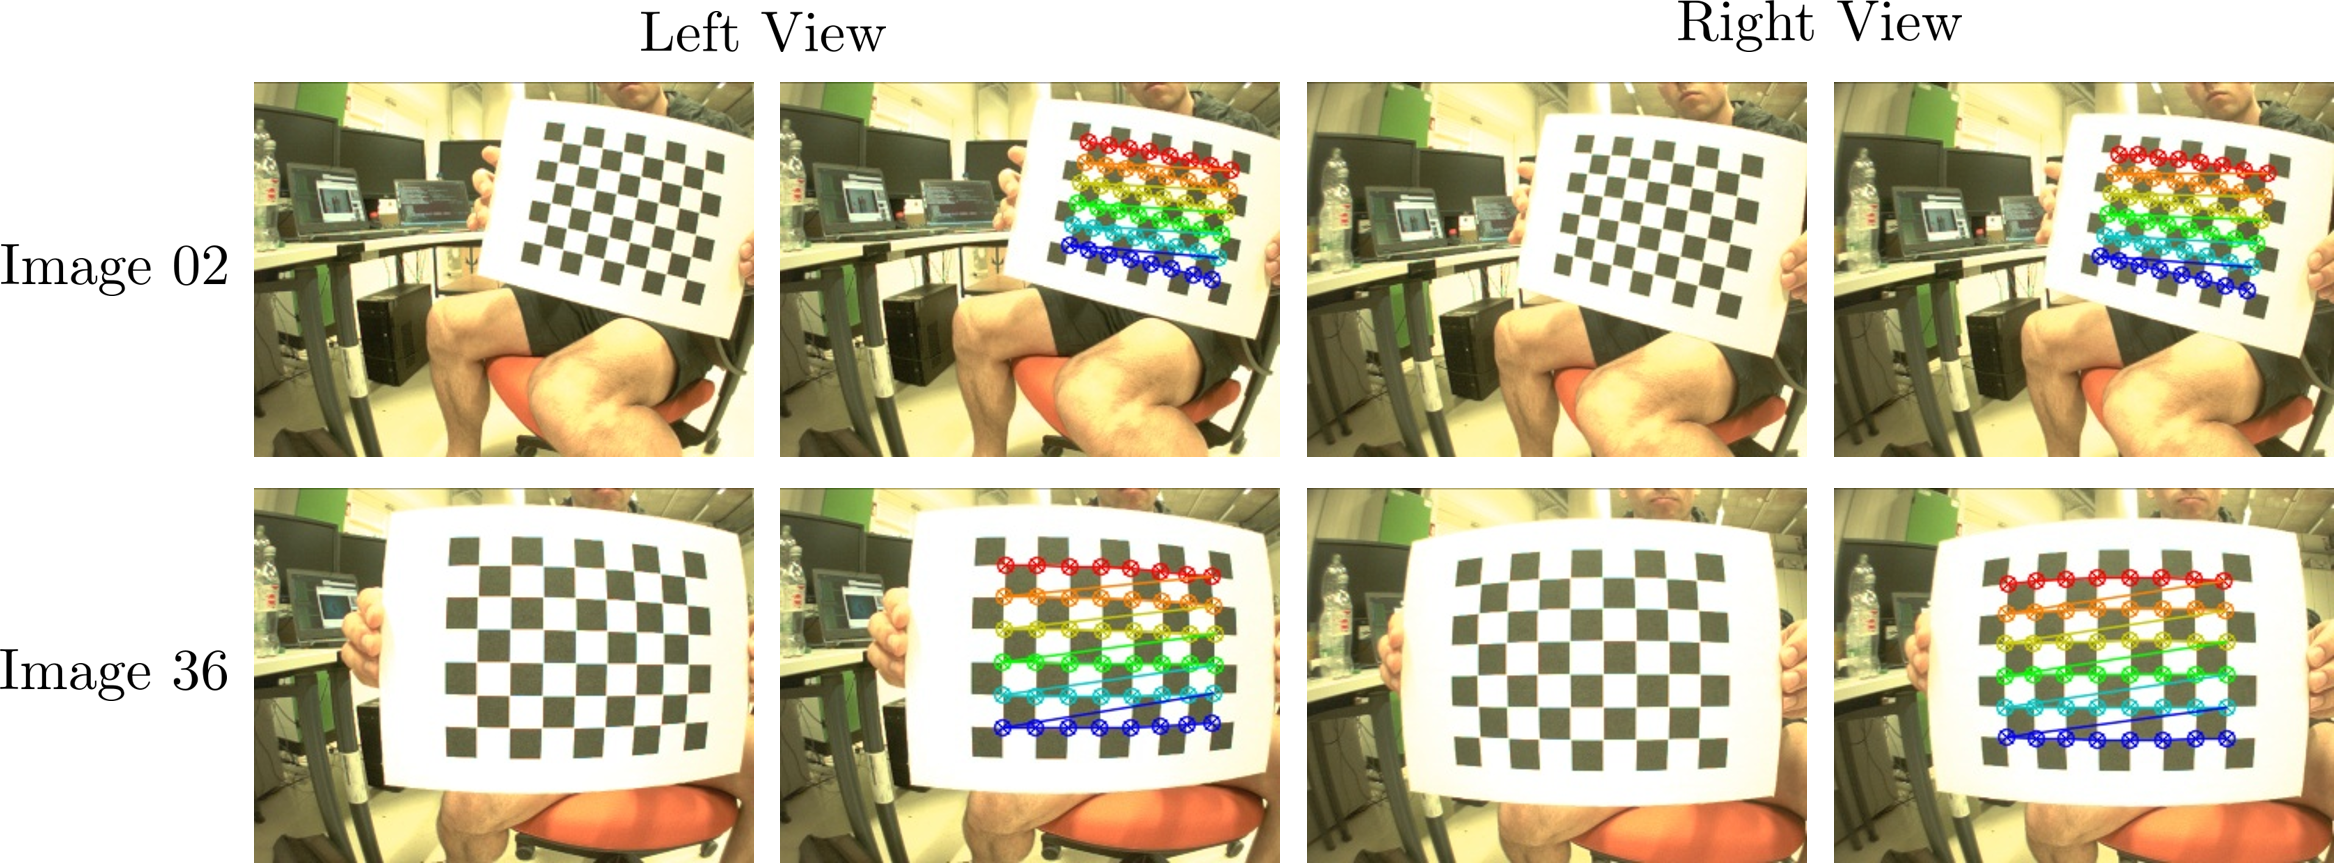
\includegraphics[scale=.28]{chapters/05_experiments/02_autonomous_walking/01_camera_calibration/calib.png}
	\caption{Exemplary left and right camera views of the calibration pattern as acquired during the calibration process. The colorful points indicate the detected corners in the image plane. Refer to figure \ref{fig::324_distortion} for the theory.}
	\label{fig::521_calib}
\end{figure}
As the resulting mean squared re-projection error $\Delta \bar{x} = 1/(WHN)\sum_0^{WHN} \Delta x$ (equation \ref{eq::324_reprojection}), we obtained $\Delta \bar{x}_l = 0.26\, \text{pixel}$, and $\Delta \bar{x}_r = 0.25\,\text{pixel}$, for the left, and the right camera, respectively. According to equations \ref{eq::324_focal_intrinsics}, \ref{eq::324_x_dist}, and \ref{eq::324_y_dist}, we therefore determined the camera intrinsic parameters as listed in table \ref{tab::521_intrinsics}.
\begin{table}[h]
	\centering
	\begin{tabular}{lll}
		Intrinsic Parameter & Left Camera & Right Camera\\
		\hline
		$f_x\,[\text{pixel}/\text{mm}]$ & $\quad2.36\cdot10^2$ & $\quad2.32\cdot10^2$ \\
		$f_y\,[\text{pixel}/\text{mm}]$ & $\quad2.37\cdot10^2$ & $\quad2.32\cdot10^2$ \\
		$c_x\,[\text{pixel}]$ & $\quad1.63\cdot10^2$ & $\quad1.86\cdot10^2$ \\
		$c_y\,[\text{pixel}]$ & $\quad1.11\cdot10^2$ & $\quad1.30\cdot10^2$ \\
		$k_1\,[1/\text{pixel}^2]$ & $-4.54\cdot10^{-1}$ & $-4.58\cdot10^{-1}$ \\
		$k_2\,[1/\text{pixel}^4]$ & $\quad2.90\cdot10^{-1}$  & $\quad3.18\cdot10^{-1}$  \\
		$k_3\,[1/\text{pixel}^6]$ & $-1.21\cdot10^{-1}$ & $-1.48\cdot10^{-1}$ \\
		$p_1\,[1/\text{pixel}]$ & $-2.73\cdot10^{-3}$ & $\quad3.02\cdot10^{-4}$  \\
		$p_2\,[1/\text{pixel}]$ & $\quad2.16\cdot10^{-4}$  & $\quad7.63\cdot10^{-4}$		
	\end{tabular}
	\caption{Intrinsic parameters of single cameras. These parameters can be found as YAML file on GitHub (\href{https://github.com/mhubii/nmpc_pattern_generator/tree/master/libs/io_module}{link}).\label{tab::521_intrinsics}}
\end{table}
Then given the calibration of each single camera, we computed the rectification transforms $\bm{R}_i$, and the projection matrices $\bm{P}_i$ in the rectified coordinate system for each camera \ref{tab::521_extrinsics}.
\begin{table}[h]
	\centering
	\begin{tabular}{lll}
		Camera & Extrinsic Parameter & \\ 
		\hline
		&& \\
		\multirow{5}{*}{Left} & $\bm{R}\,[\text{a.u.}]$              & $\begin{pmatrix}
		\quad9.93\cdot10^{-1} & -2.65\cdot10^{-3}     & \quad1.14\cdot10^{-1} \\ 
		\quad5.41\cdot10^{-1} & \quad1.00\cdot10^{0}  & -2.39\cdot10^{-2} \\
		-1.14\cdot10^{-1}     & \quad2.43\cdot10^{-2} & \quad9.93\cdot10^{-1}
		\end{pmatrix}$ \\&&\\
		& $\bm{P}\,[\text{pixel}/\text{mm}]$              & $\begin{pmatrix}
		2.34\cdot10^{2} & 0.00     & 1.88\cdot10^{2} & 0.00\,\text{mm} \\ 
		0.00 & 2.34\cdot10^{2}  & 4.87\cdot10^{1} & 0.00\,\text{mm} \\
		0.00    & 0.00 & 1.00 & 0.00\,\text{mm}
		\end{pmatrix}$ \\
		&&\\
		\multirow{5}{*}{Right} & $\bm{R}\,[\text{a.u.}]$              & $\begin{pmatrix}
		\quad9.95\cdot10^{-1} & -2.30\cdot10^{-2}     & \quad9.93\cdot10^{-2} \\ 
		\quad2.07\cdot10^{-2} & \quad1.00\cdot10^{0}  & \quad2.38\cdot10^{-2} \\
		-9.98\cdot10^{-2}     & -2.16\cdot10^{-2} & \quad9.95\cdot10^{-1}
		\end{pmatrix}$ \\&&\\
		& $\bm{P}\,[\text{pixel}/\text{mm}]$              & $\begin{pmatrix}
		2.34\cdot10^{2} & 0.00     & 1.88\cdot10^{2} & -1.60\cdot10^1\,\text{mm} \\ 
		0.00 & 2.34\cdot10^{2}  & 4.88\cdot10^{1} & 0.00\,\text{mm} \\
		0.00    & 0.00 & 1.00 & 0.00\,\text{mm}
		\end{pmatrix}$ \\
	\end{tabular}
	\caption{Rectification transforms $\bm{R}_i$, and projection matrices $\bm{P}_i$, for the left, and the right camera, respectively. These parameters can be found as YAML file on GitHub (\href{https://github.com/mhubii/nmpc_pattern_generator/blob/master/libs/io_module/cam_stereo.yaml}{link}). \label{tab::521_extrinsics}}
\end{table}
Exemplary rectified images, which rely on the matrices of table \ref{tab::521_extrinsics}, are shown in figure \ref{fig::521_rect} (a). Since there is a slight rotation of the calibration pattern, it is not obvious that the images got rectified well. Therefore, the same images are shown in figure \ref{fig::521_rect} (b), but slightly rotated such that the calibration pattern aligns horizontally. The blue line therein indicates that in contrast to the original image, straight lines now appear straight across both images, which is crucial for the block matching algorithm in the next section - Depth Map Parameter Tuning.
\begin{figure}[h]
	\centering
	\subcaptionbox{Rectified images.}%
	[.4\linewidth]{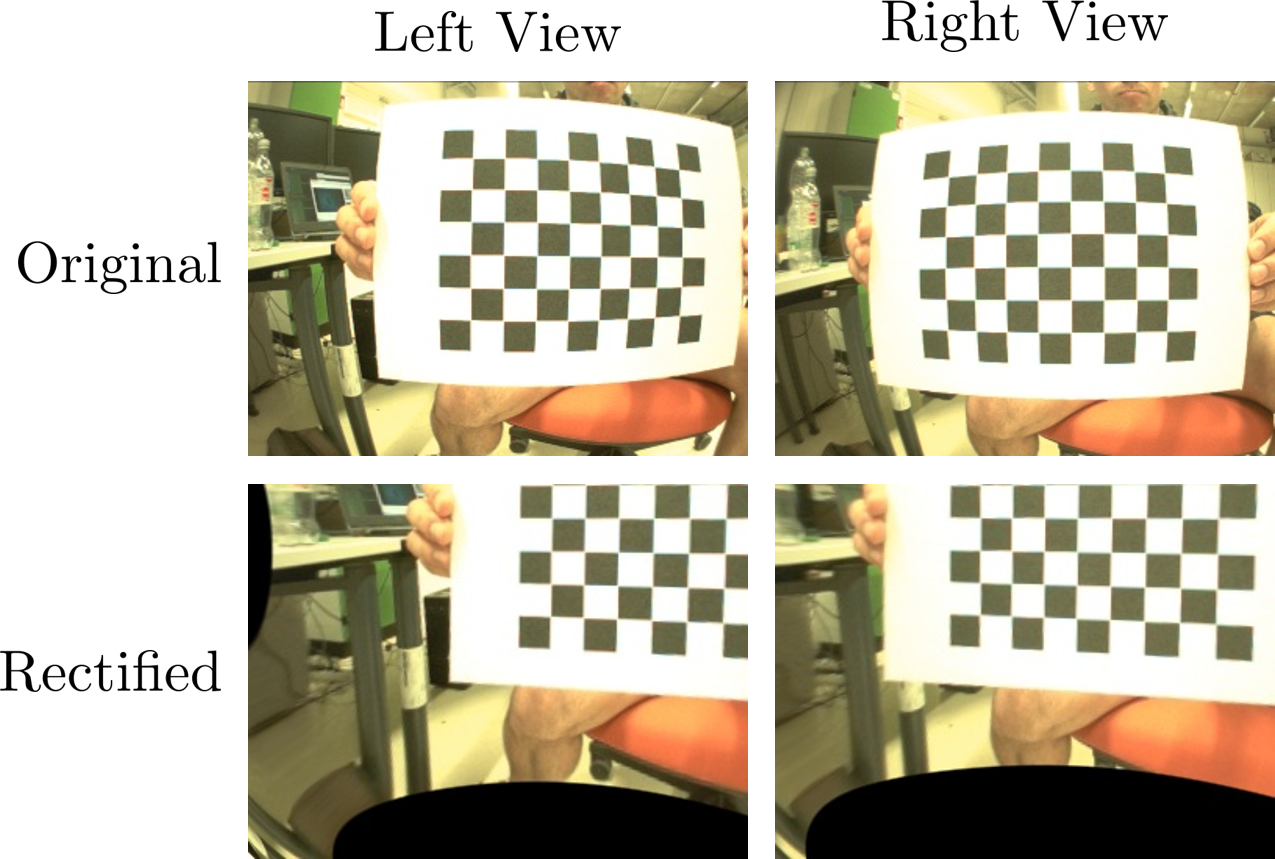
\includegraphics[scale=.25]{chapters/05_experiments/02_autonomous_walking/01_camera_calibration/rect.png}}
	\subcaptionbox{Rotated rectified images.}%
	[.4\linewidth]{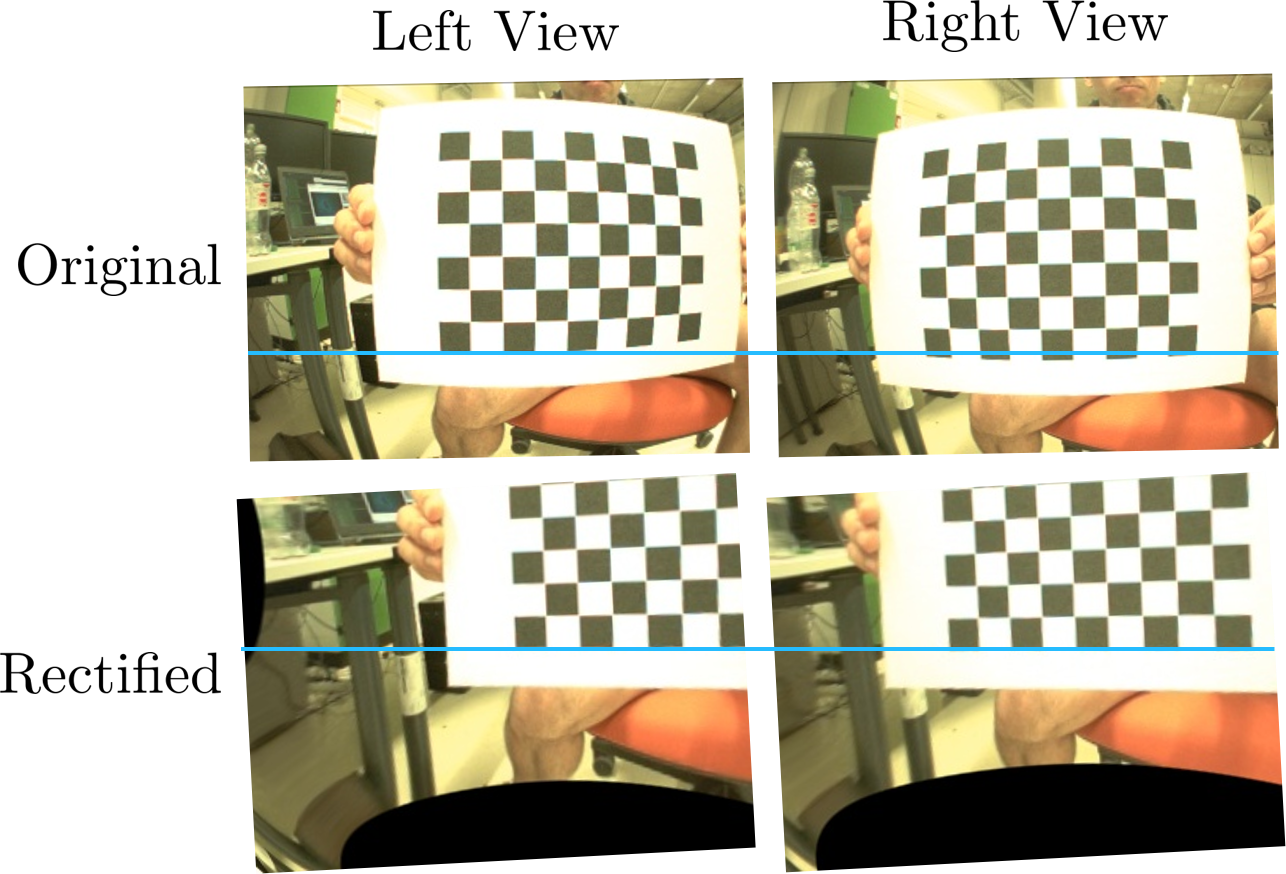
\includegraphics[scale=.25]{chapters/05_experiments/02_autonomous_walking/01_camera_calibration/rect_line.png}}
	\caption{Rectified and original view of the stereo camera. Refer to figure \ref{fig::324_rectified} for the theory.}
	\label{fig::521_rect}
\end{figure}
\subsection{Depth Parameter Tuning}
Within this section, we shortly explore the effects of all tunable parameters on the depth map generation. Therefore, we utilize a simple experimental setup. Within the setup, Heicub points its stereo camera towards three chairs that are located at a distance of $1\,\text{m}$ towards each other, and towards the cameras, so to cover close, medium, and far distances. The consecutive chairs are slightly shifted, in order to enable the simultaneous observation of all of them. The rectified view of the environment is shown in figure \ref{fig::522_wls_rgb}.
\begin{figure}[h]
	\centering
	\subcaptionbox{Left camera's view.}%
	[.4\linewidth]{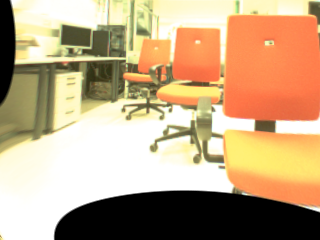
\includegraphics[scale=.3]{chapters/05_experiments/02_autonomous_walking/02_depth_map_parameter_tuning/l_rgb.png}}
	\subcaptionbox{Right camera's view.}%
	[.4\linewidth]{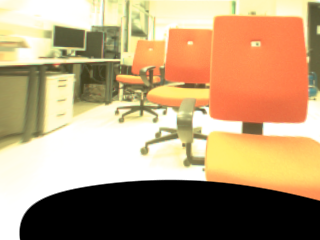
\includegraphics[scale=.3]{chapters/05_experiments/02_autonomous_walking/02_depth_map_parameter_tuning/r_rgb.png}}
	\caption{Heicub's perspective of the scene for the depth map parameter tuning.}
	\label{fig::522_wls_rgb}
\end{figure}
The depth map extraction, which utilizes the rectified images, depends on a stereo block matching algorithm that got explained in section \ref{sec::324_ip}. It mainly depends on the window size and the number of disparities for the sum of absolute difference computation. We evaluate the influence of those two parameters in figure \ref{fig::522_disp} (a) in a grid search fashion. It is apparent that the change in the number of disparities has close to no influence onto the depth map quality, while it removes plenty of useful information from the left hand side of images. The same holds true for the window size, except that it removes some noise from the depth maps.
\begin{figure}[h]
	\centering
	\subcaptionbox{Left disparity. Please refer to figure \ref{fig::324_left_disparity_map} and equation \ref{eq::324_sad} for the theory.}%
	[.45\linewidth]{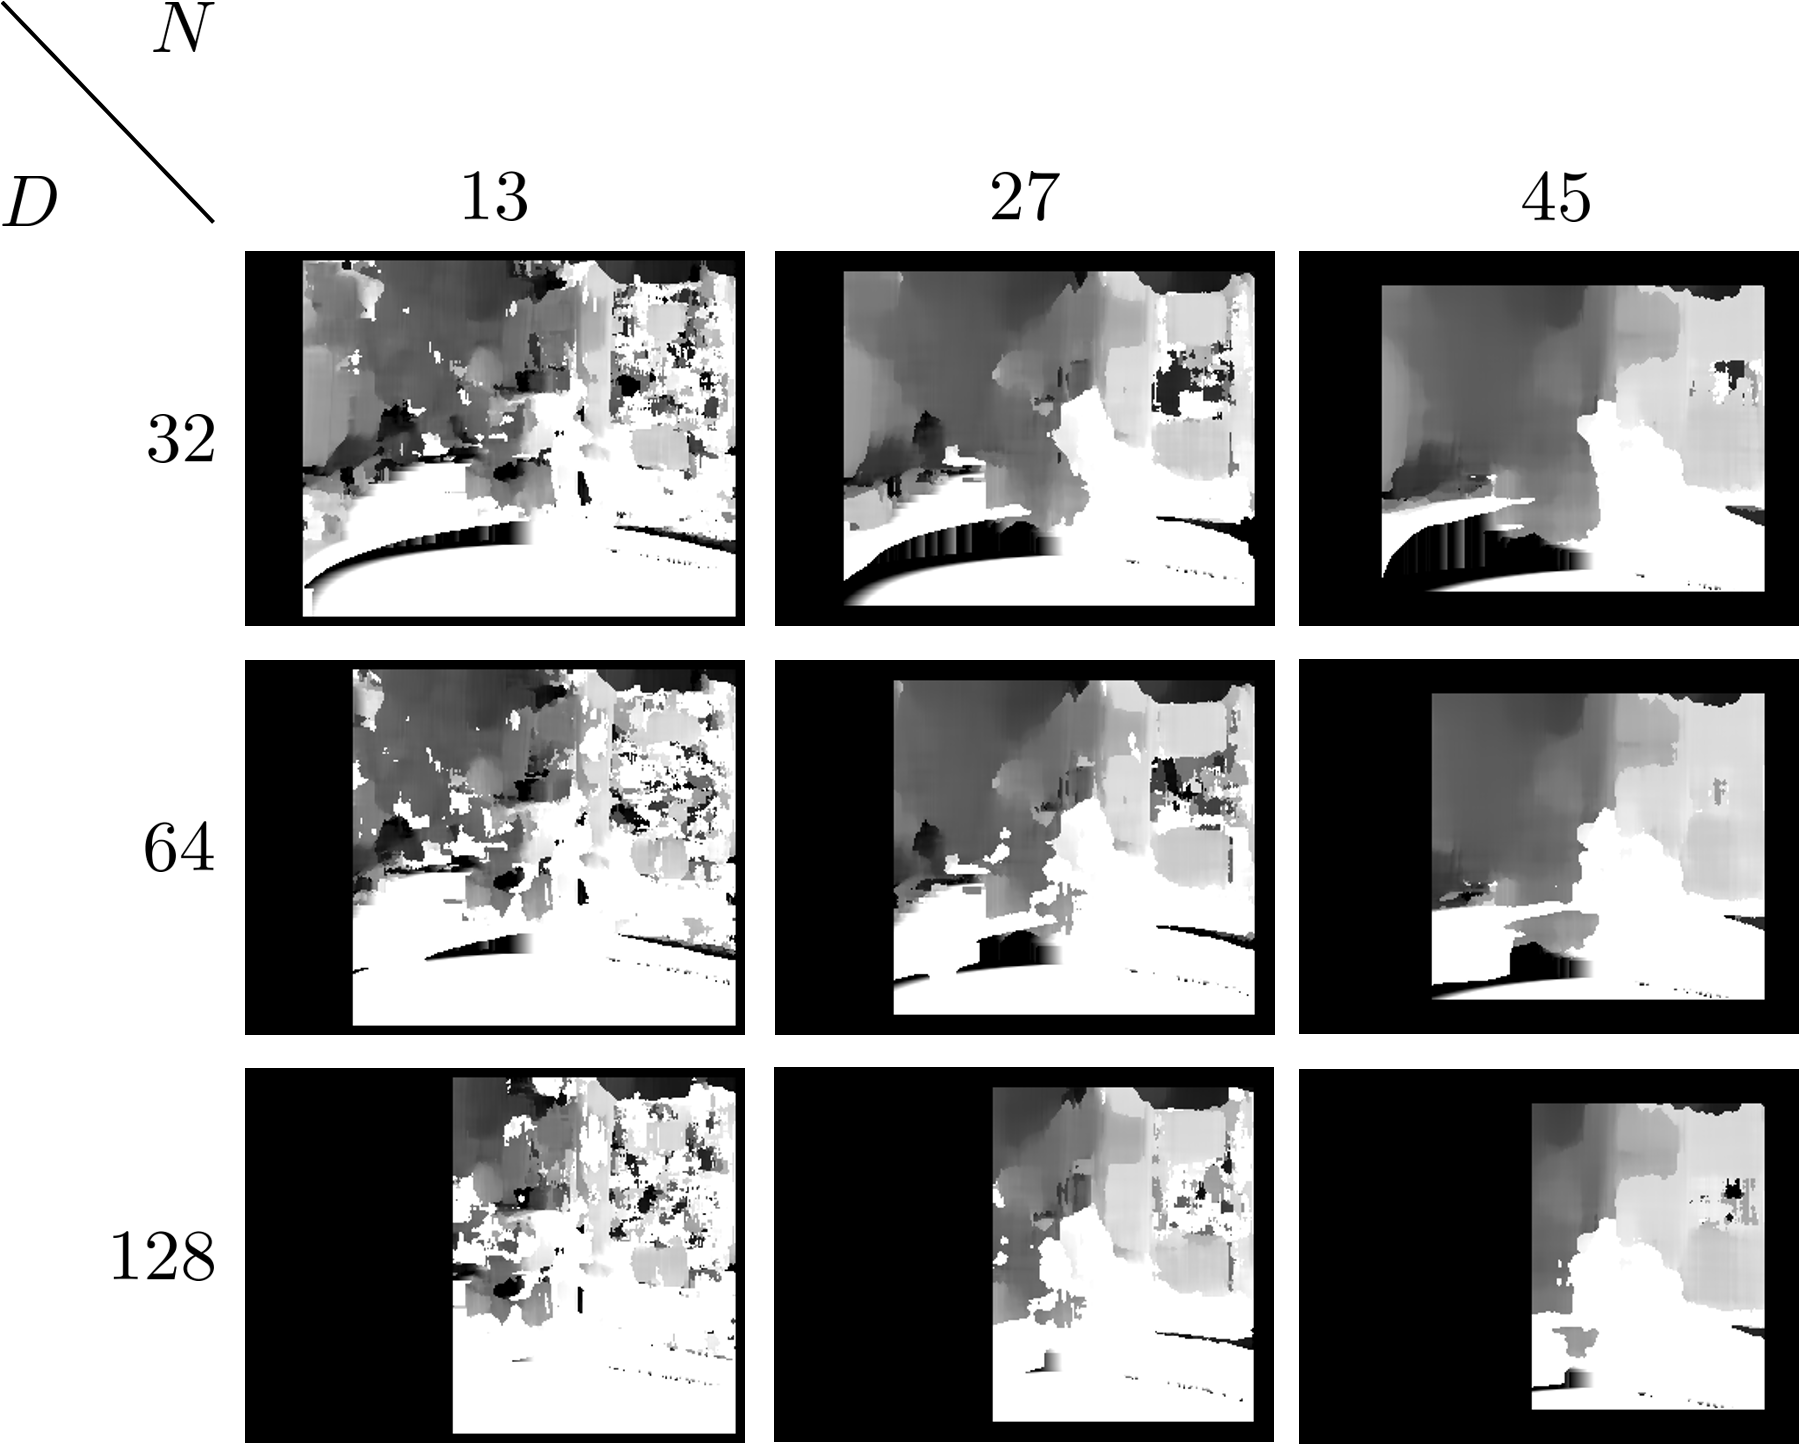
\includegraphics[scale=.2]{chapters/05_experiments/02_autonomous_walking/02_depth_map_parameter_tuning/disp_sad.png}}
	\subcaptionbox{Confidence weighted least squares disparity map. Please refer to figure \ref{fig::324_weighted_least_squares_disparity} and equation \ref{eq::324_wls_final} for the theory.}%
	[.45\linewidth]{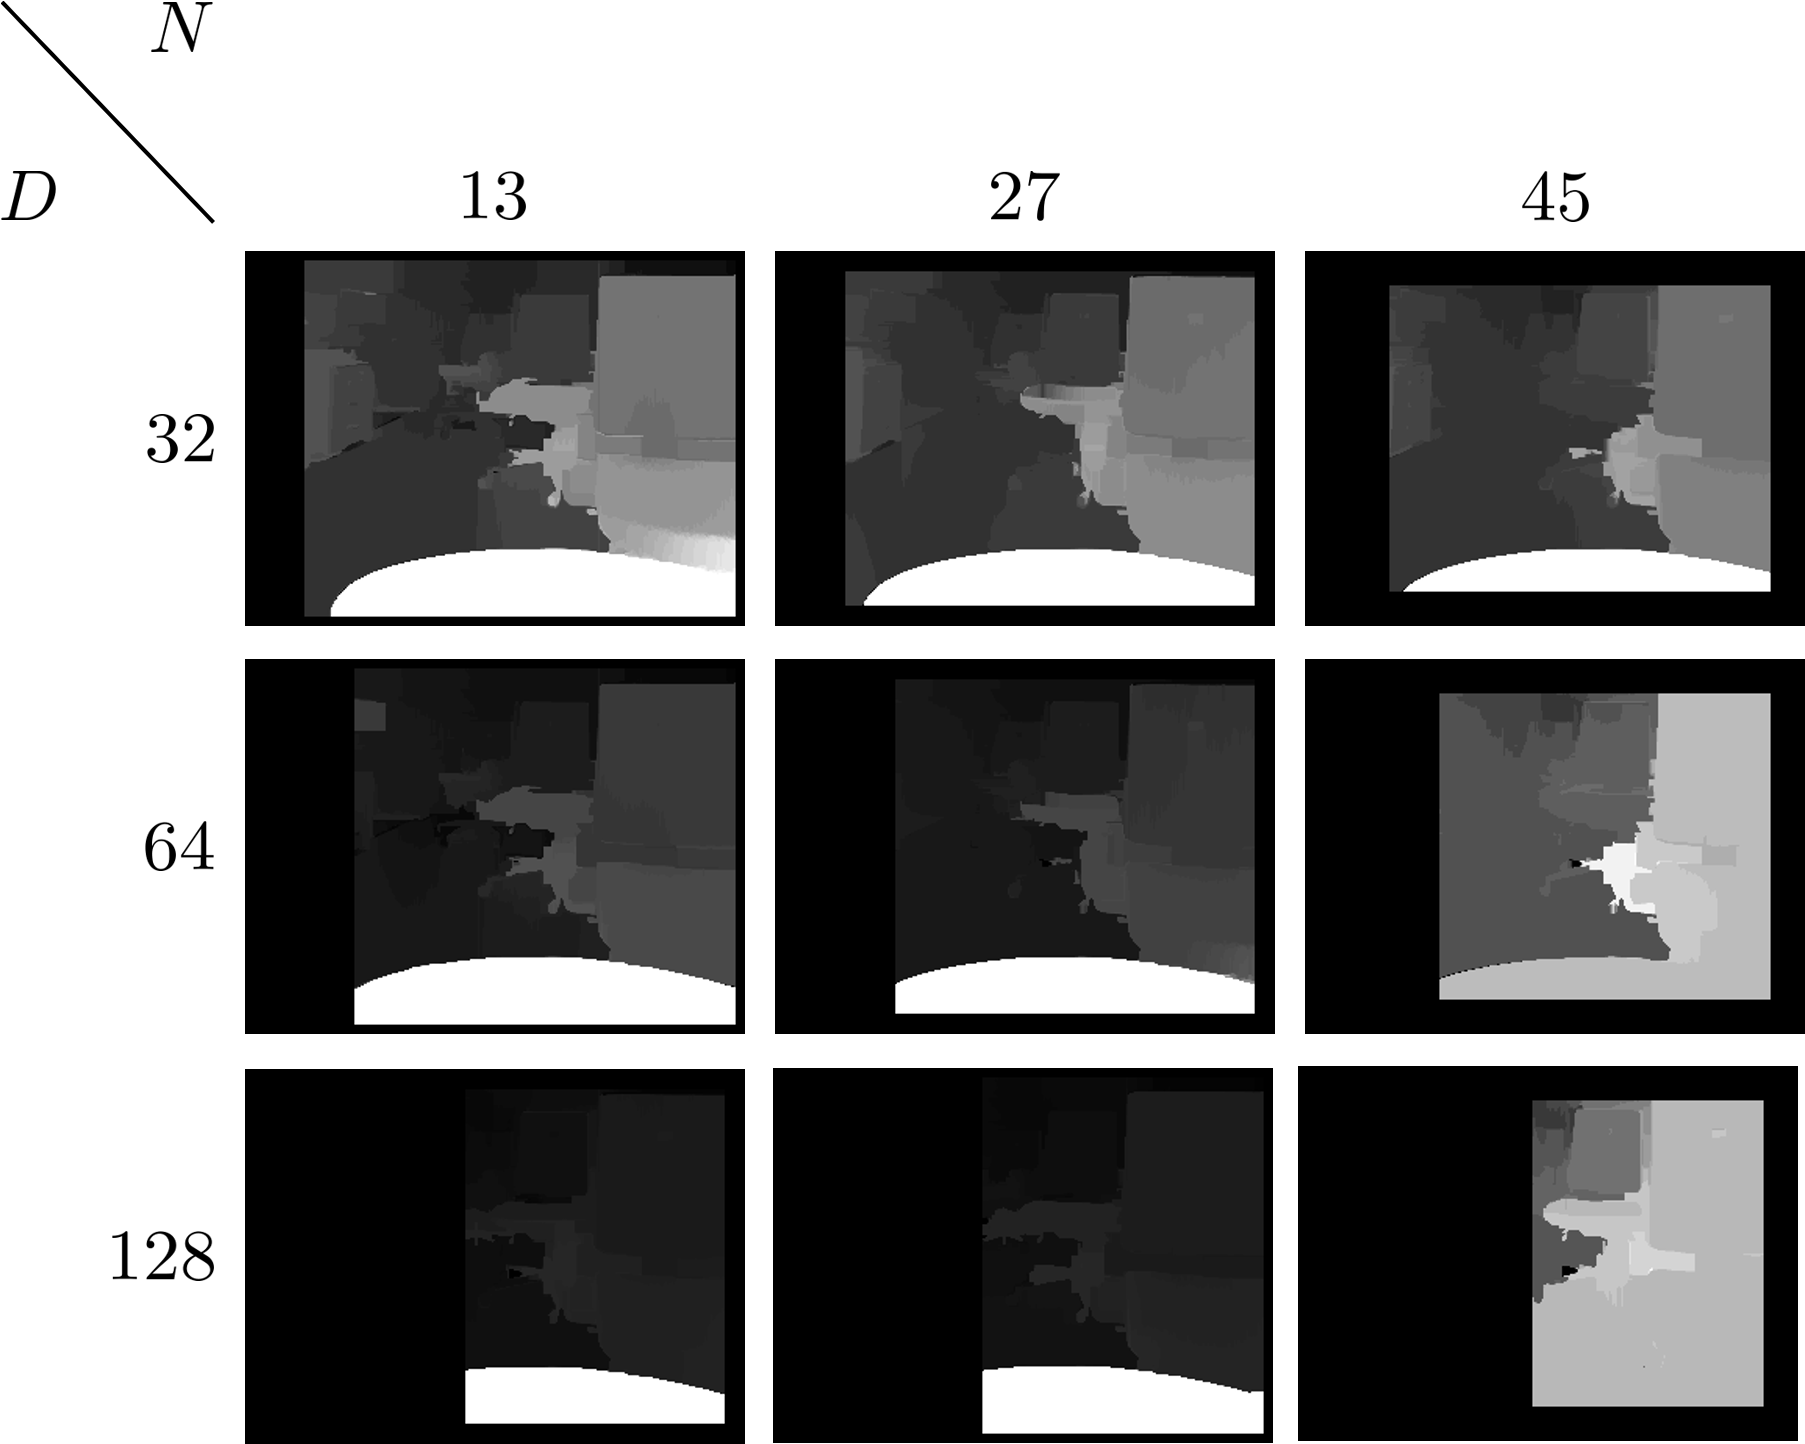
\includegraphics[scale=.2]{chapters/05_experiments/02_autonomous_walking/02_depth_map_parameter_tuning/disp_sad_wls.png}}
	\caption{Left disparity map and confidence weighted least squares disparity for changing SAD window sizes $N$ and number of disparities $D$.}
	\label{fig::522_disp}
\end{figure}
In combination with the confidence weighted least squares filtering, we can observe that most of the noise is already removed (figure \ref{fig::522_disp} (b)), for which it is more import to keep the information close to the images' borders. We therefore chose to set the number of disparities $D=32$, and the windows size $N=13$ in the following. Within these depth maps, the global energy weighting $\lambda$ was set to $10^4$, and the local bilateral filter decay $\sigma$ to $1$, since we observed the best performance for them. The influence of those two parameters is visualized in figure \ref{fig::522_sigma_lambda}. We can see that, in good accordance with the theory, $\sigma$ contributes to the smoothing of the depth map, and that $\lambda$ enforces a change in depth across edges within the RGB images.
\begin{figure}[h]
	\centering
	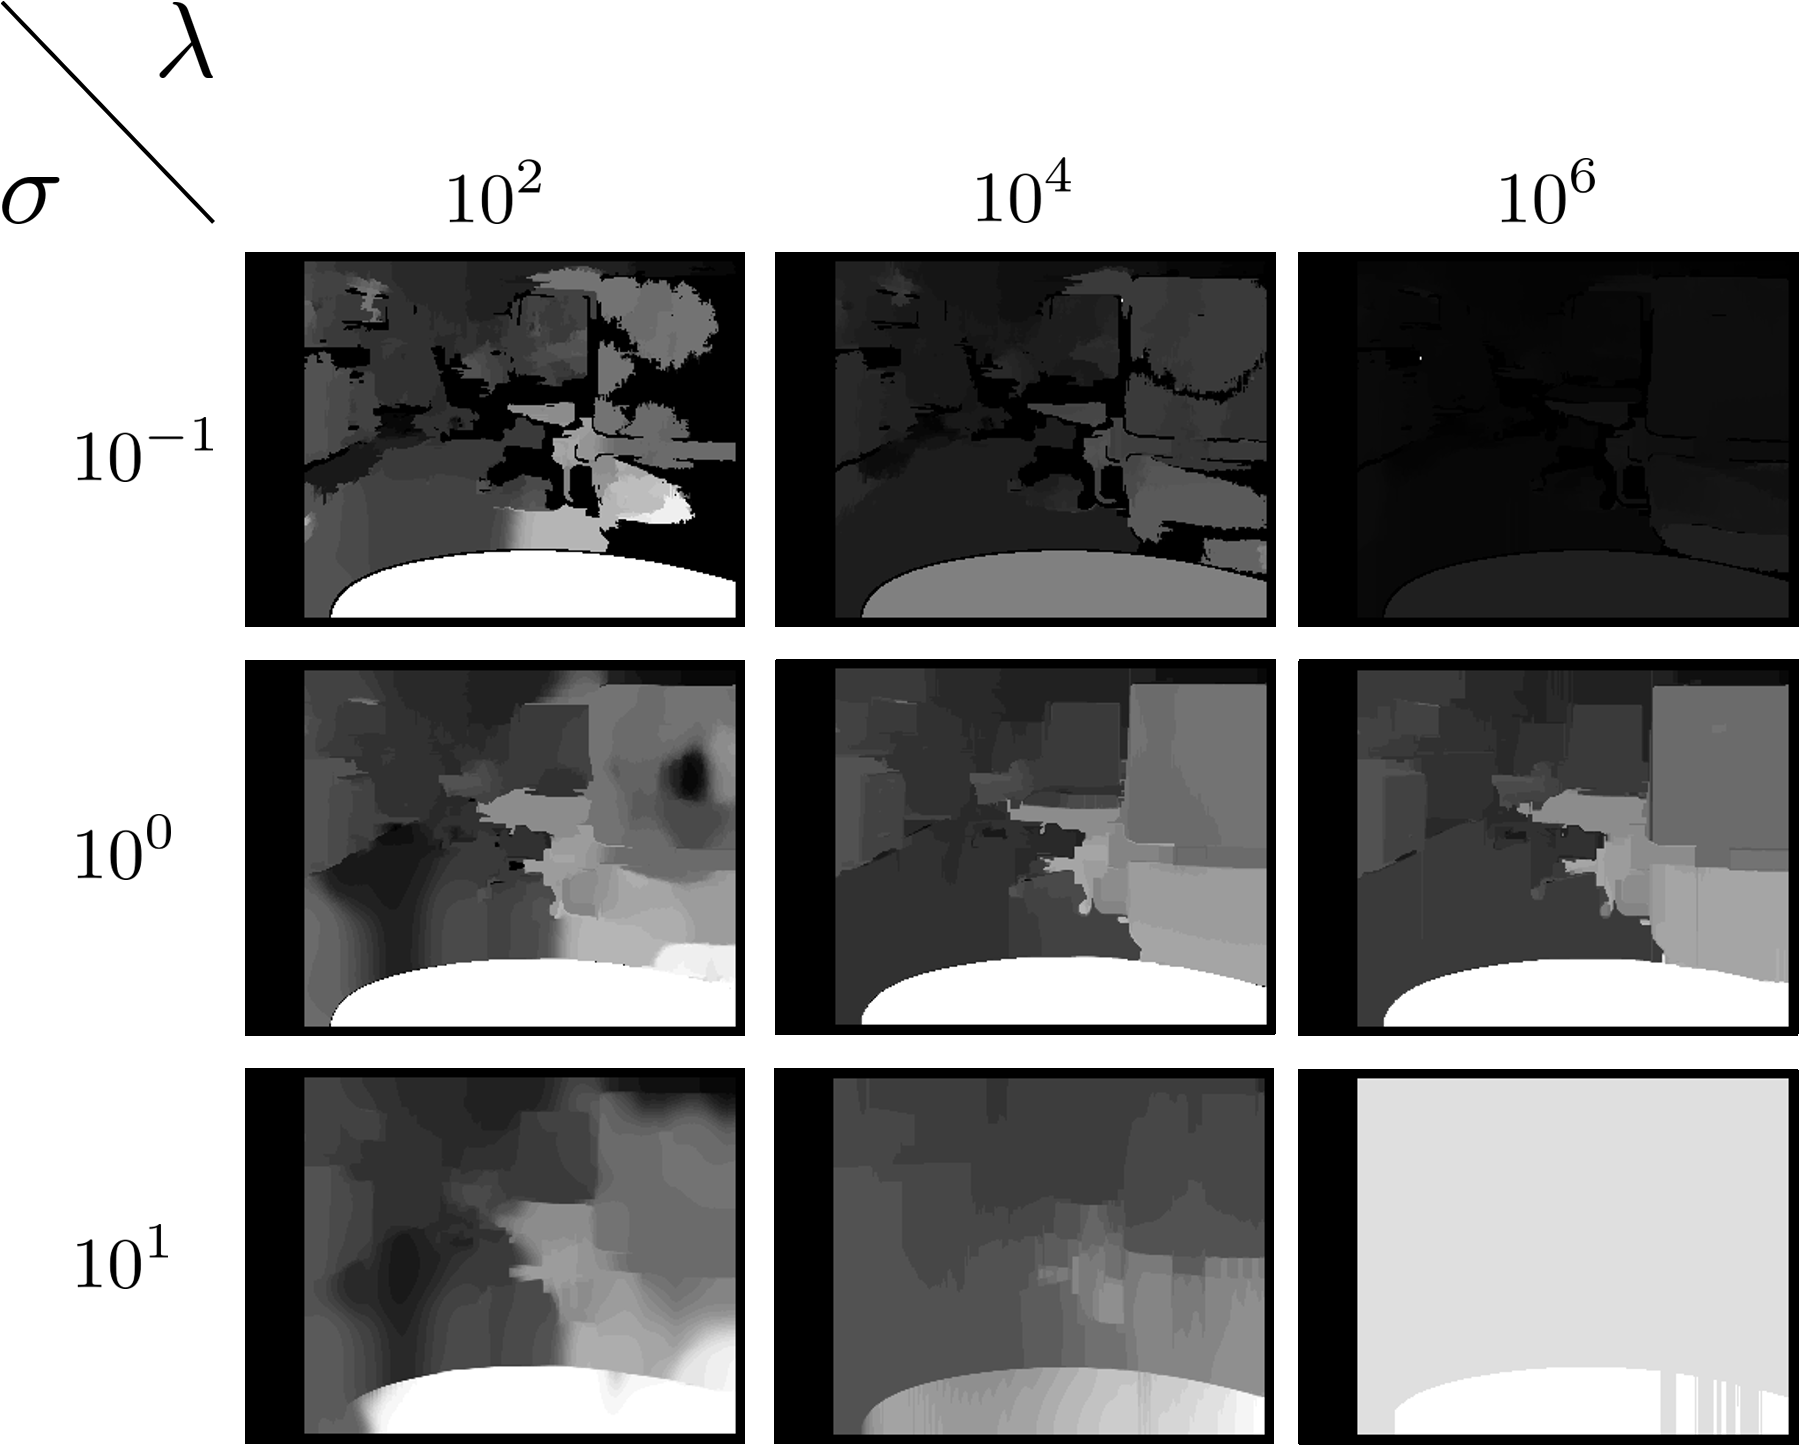
\includegraphics[scale=.2]{chapters/05_experiments/02_autonomous_walking/02_depth_map_parameter_tuning/sigma_lambda.png}
	\caption{Confidence weighted least squares disparity for changing energy weightings $\sigma$ and $\lambda$. Please refer to equations \ref{eq::324_weight} and \ref{eq::324_energy_function} for the theory.}
	\label{fig::522_sigma_lambda}
\end{figure}
\subsection{Data Acquisition}
\label{sec::523_da}

\begin{figure}[h]
	\centering
	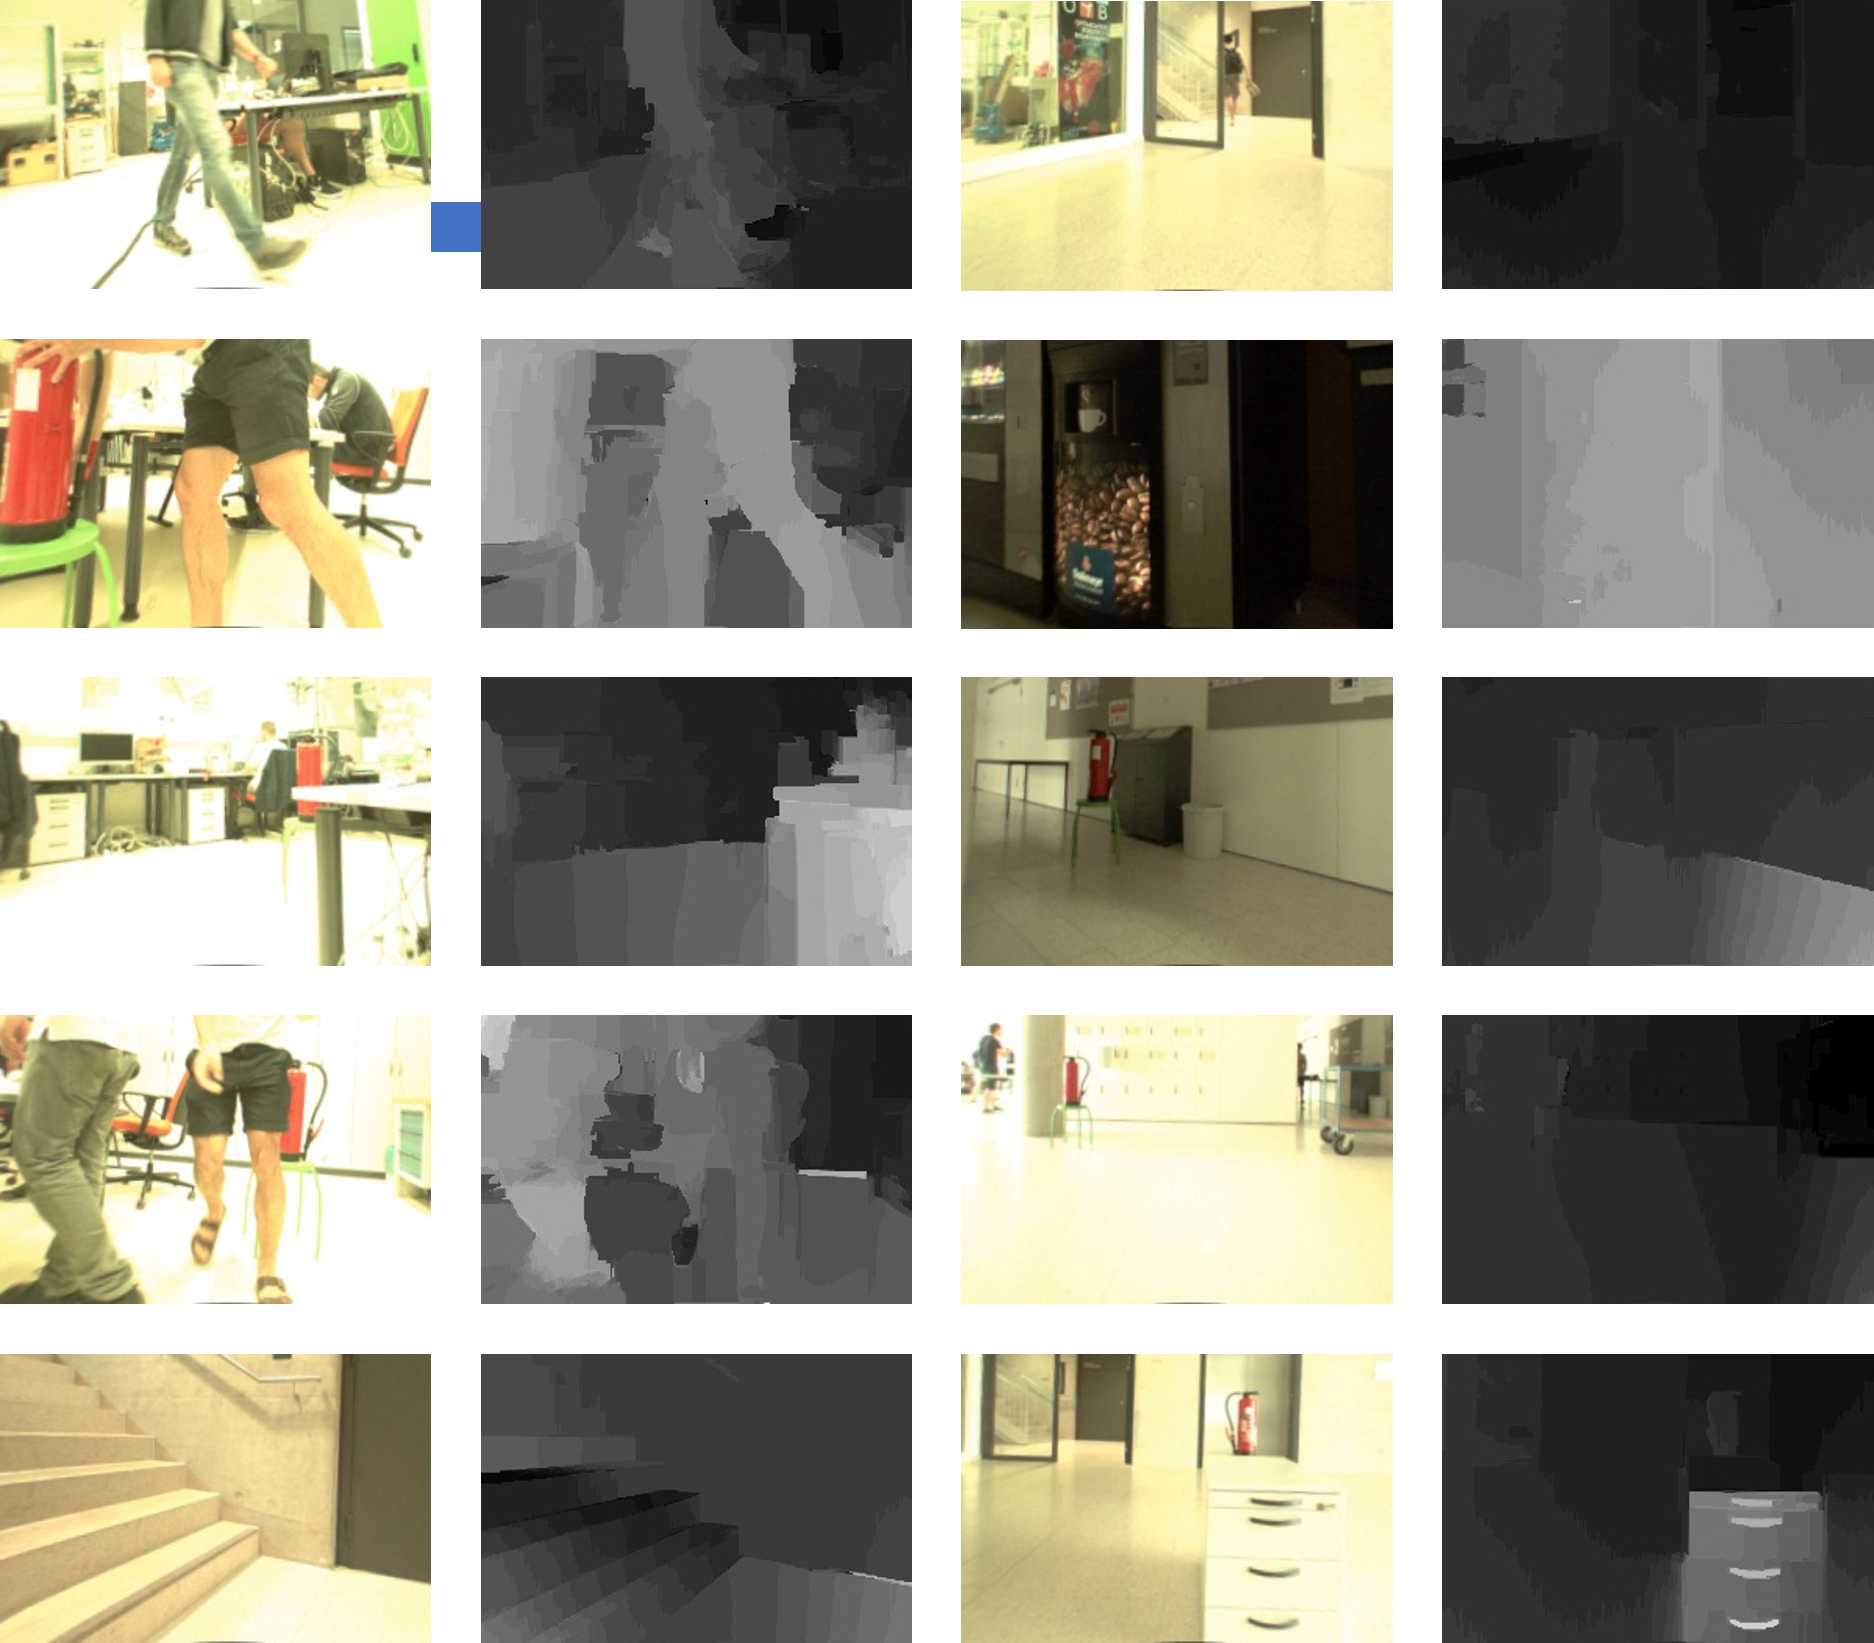
\includegraphics[scale=.4]{chapters/05_experiments/02_autonomous_walking/dataset_diversity.png}
	\caption{}
	\label{fig::523_dataset}
\end{figure}
\subsection{Network Training}
\begin{figure}[h]
	\centering
	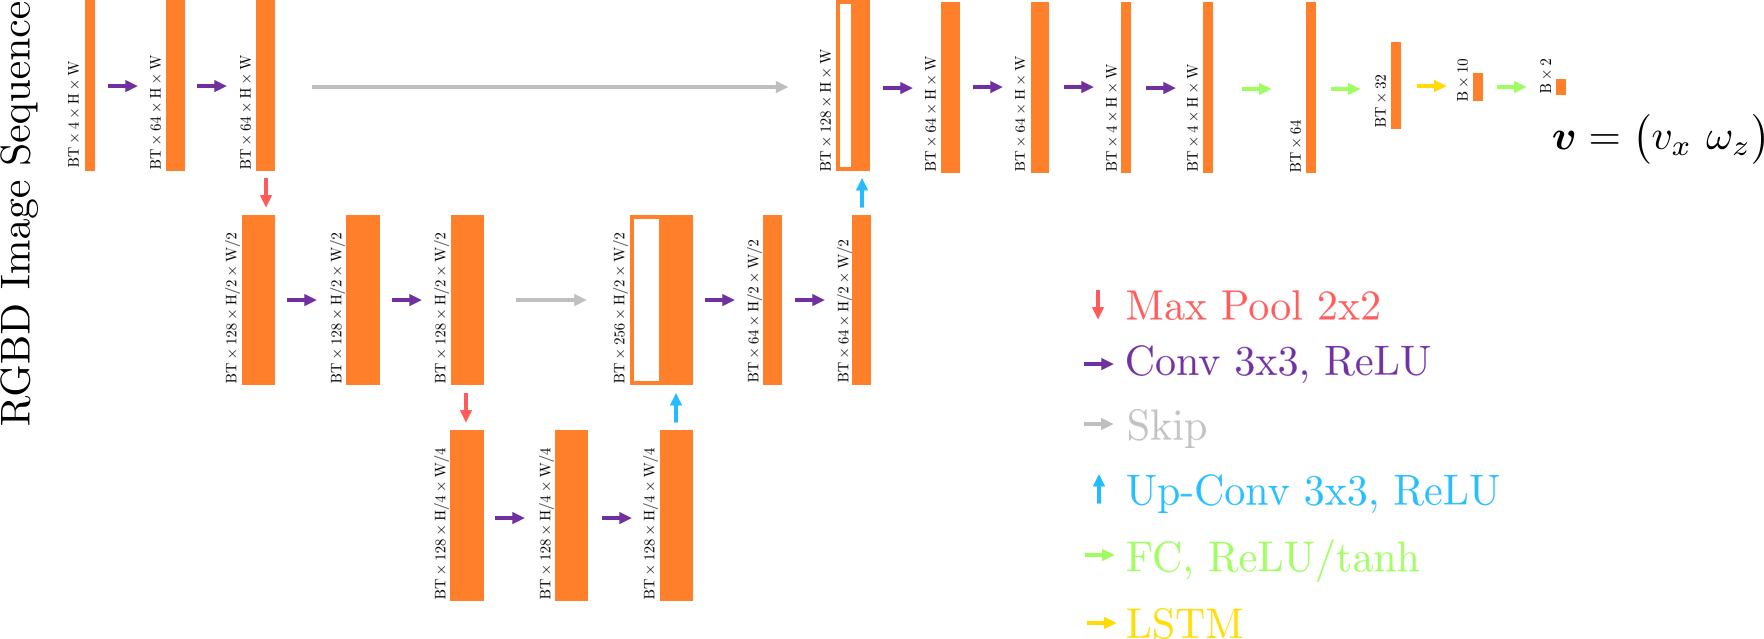
\includegraphics[scale=.5]{chapters/05_experiments/02_autonomous_walking/unet.png}
	\caption{}
	\label{fig::524_unet}
\end{figure}
\begin{figure}[h]
	\centering
	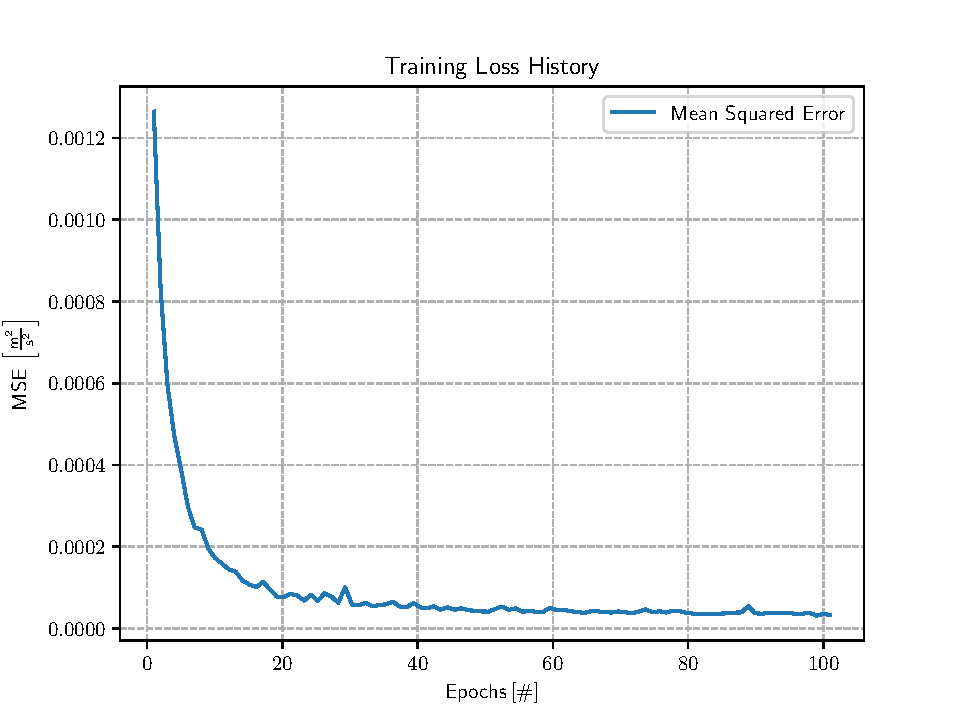
\includegraphics[scale=.6]{chapters/05_experiments/02_autonomous_walking/05_07_19_loss_history.pdf}
	\caption{}
	\label{fig::524_loss}
\end{figure}
\begin{figure}[h]
	\centering
	\subcaptionbox{}%
	[.4\linewidth]{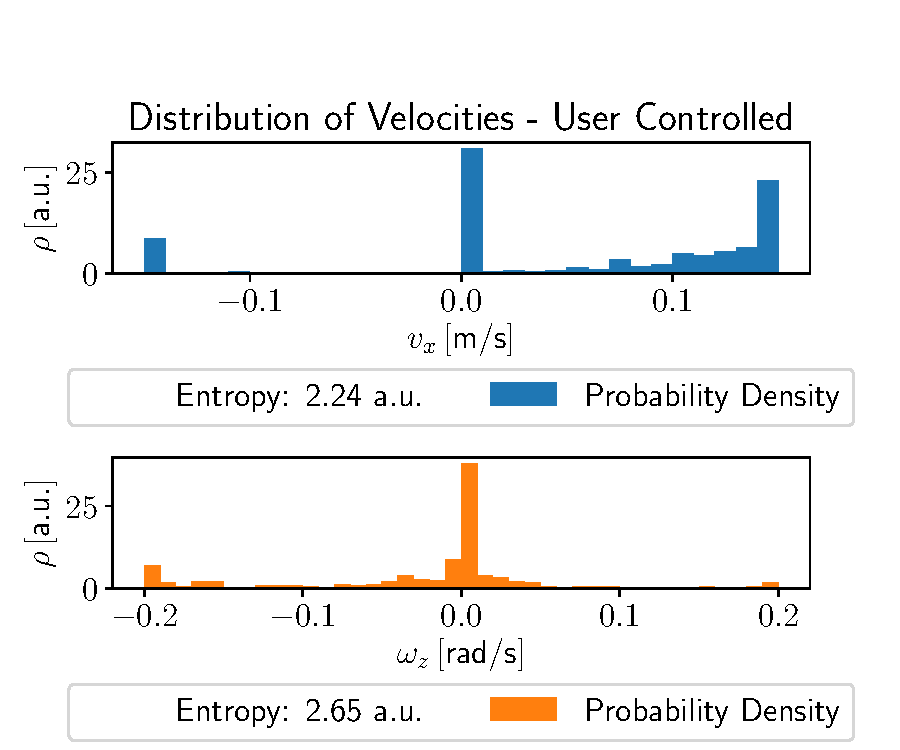
\includegraphics[scale=.35]{chapters/05_experiments/02_autonomous_walking/user_entropy.pdf}}
	\subcaptionbox{}%
	[.4\linewidth]{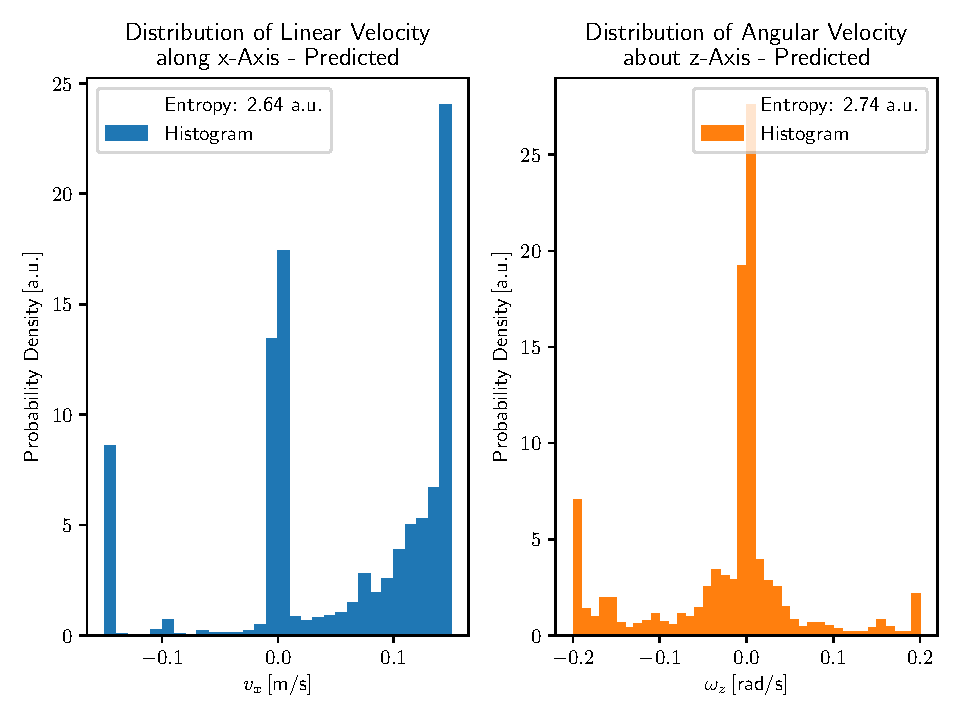
\includegraphics[scale=.35]{chapters/05_experiments/02_autonomous_walking/predicted_entropy_kldivx_0_33_kldivz_0_06_imgs_13441_duration_4_ms.pdf}}
	\caption{KL divergence x 0.33, KL divergence z 0.06, validation split on 13441 imgs, average duration 4 ms}
	\label{fig::524_training_dist}
\end{figure}
% compute kl divergence for whole set -> argue that this holds true for all 
\subsection{Performance in Test Environment}
\begin{figure}[h]
	\centering
	\subcaptionbox{Straight Walk}%
	[.4\linewidth]{\animategraphics[height=1.2in,loop,autoplay]{20}{chapters/05_experiments/02_autonomous_walking/straight_walk_01/frame-}{001}{033}}
	\subcaptionbox{Curved Walk}%
	[.4\linewidth]{\animategraphics[height=1.2in,loop,autoplay]{20}{chapters/05_experiments/02_autonomous_walking/curved_walk_02/frame-}{001}{039}}
	\subcaptionbox{Obstacle Avoidance}%
	[.4\linewidth]{\animategraphics[height=1.2in,loop,autoplay]{20}{chapters/05_experiments/02_autonomous_walking/obstacle_walk_02/frame-}{001}{017}}
	\subcaptionbox{Environment Scanning}%
	[.4\linewidth]{\animategraphics[height=1.2in,loop,autoplay]{20}{chapters/05_experiments/02_autonomous_walking/out_of_sight_walk_01/frame-}{001}{075}}
	\caption{}
	\label{fig::525_aw_gif_basic}
\end{figure} 
\begin{figure}[h]
	\centering
	\subcaptionbox{Straight Walk - Dynamic Balance}%
	[.4\linewidth]{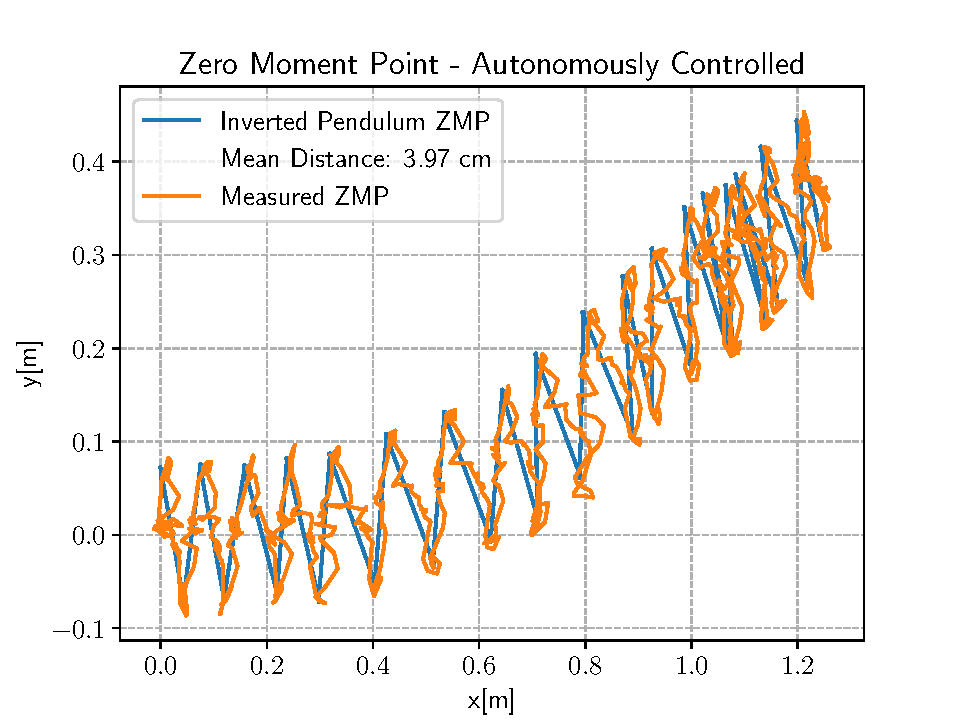
\includegraphics[scale=.35]{chapters/05_experiments/02_autonomous_walking/straight_walk_01_zmp.pdf}}
	\subcaptionbox{Straight Walk - Behavior}%
	[.4\linewidth]{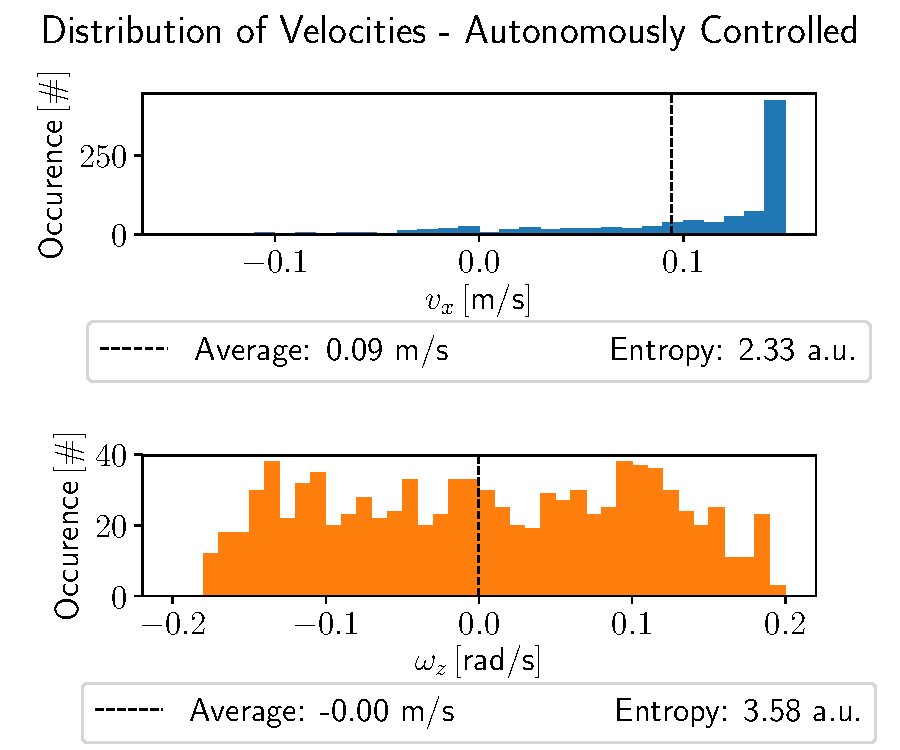
\includegraphics[scale=.35]{chapters/05_experiments/02_autonomous_walking/straight_walk_01_entropy.pdf}}
	\subcaptionbox{Curved Walk - Dynamic Balance}%
	[.4\linewidth]{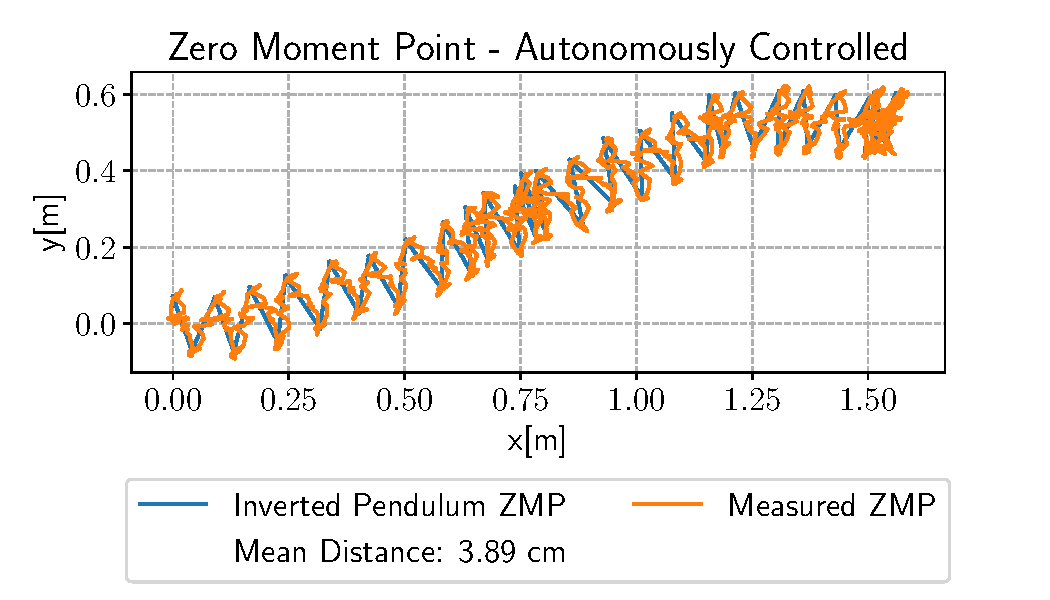
\includegraphics[scale=.35]{chapters/05_experiments/02_autonomous_walking/curved_walk_01_zmp.pdf}}
	\subcaptionbox{Curved Walk - Behavior}%
	[.4\linewidth]{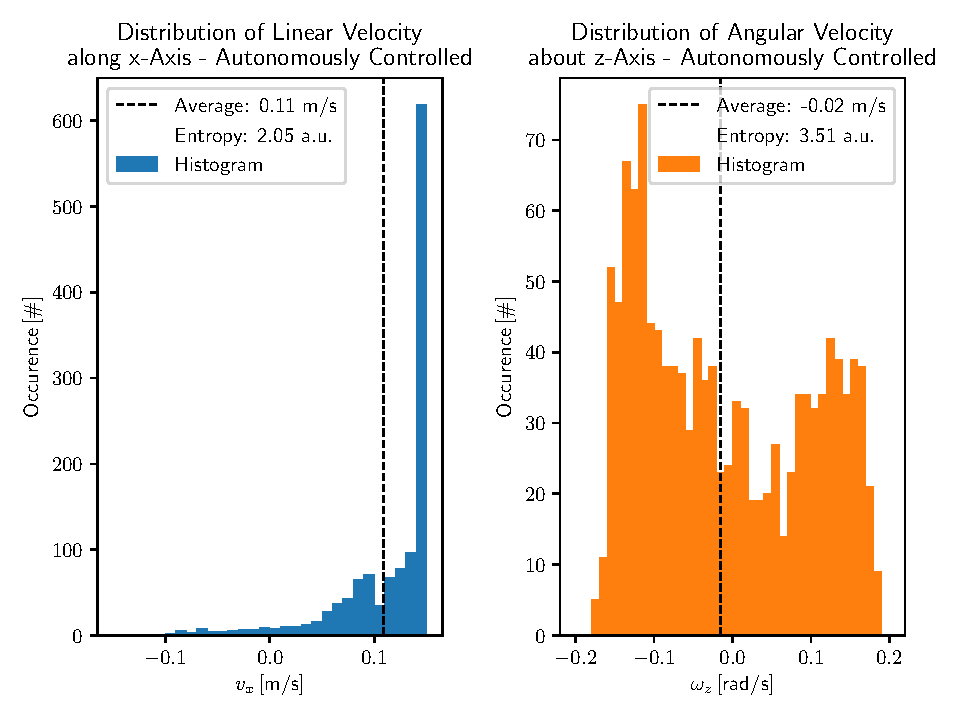
\includegraphics[scale=.35]{chapters/05_experiments/02_autonomous_walking/curved_walk_01_entropy.pdf}}
	\subcaptionbox{Obstacle Avoidance - Dynamic Balance}%
	[.4\linewidth]{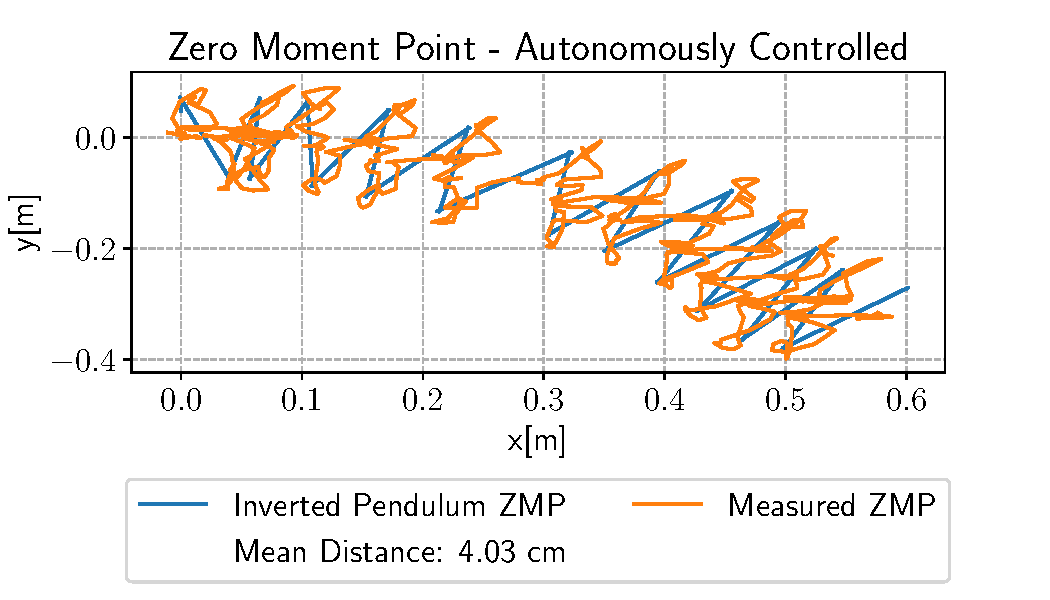
\includegraphics[scale=.35]{chapters/05_experiments/02_autonomous_walking/obstacle_walk_02_zmp.pdf}}
	\subcaptionbox{Obstacle Avoidance - Behavior}%
	[.4\linewidth]{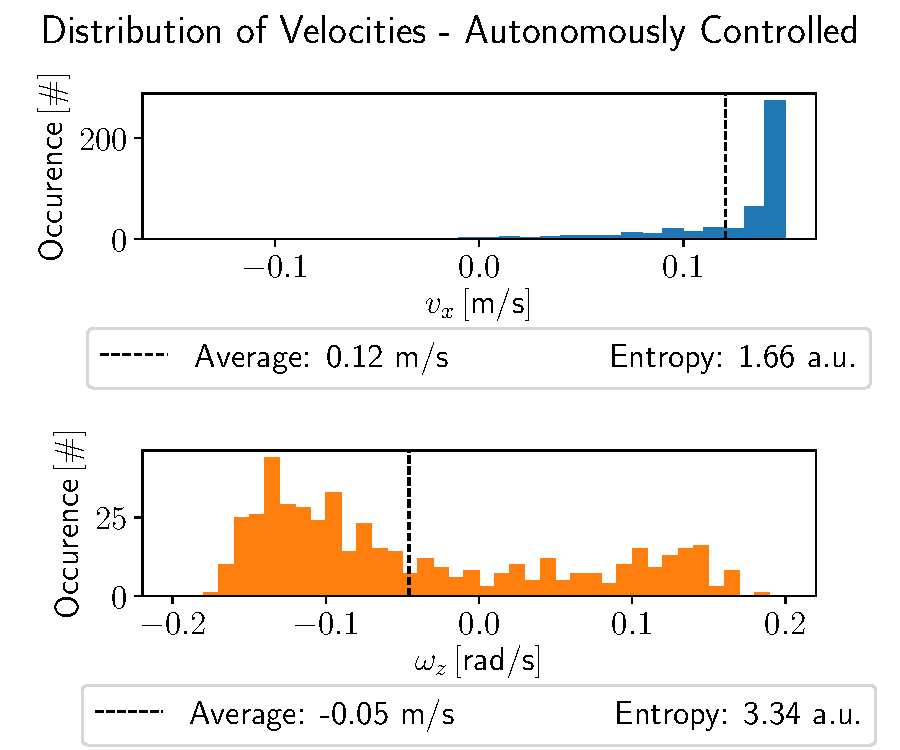
\includegraphics[scale=.35]{chapters/05_experiments/02_autonomous_walking/obstacle_walk_02_entropy.pdf}}
	\subcaptionbox{Environment Scanning - Dynamic Balance}%
	[.4\linewidth]{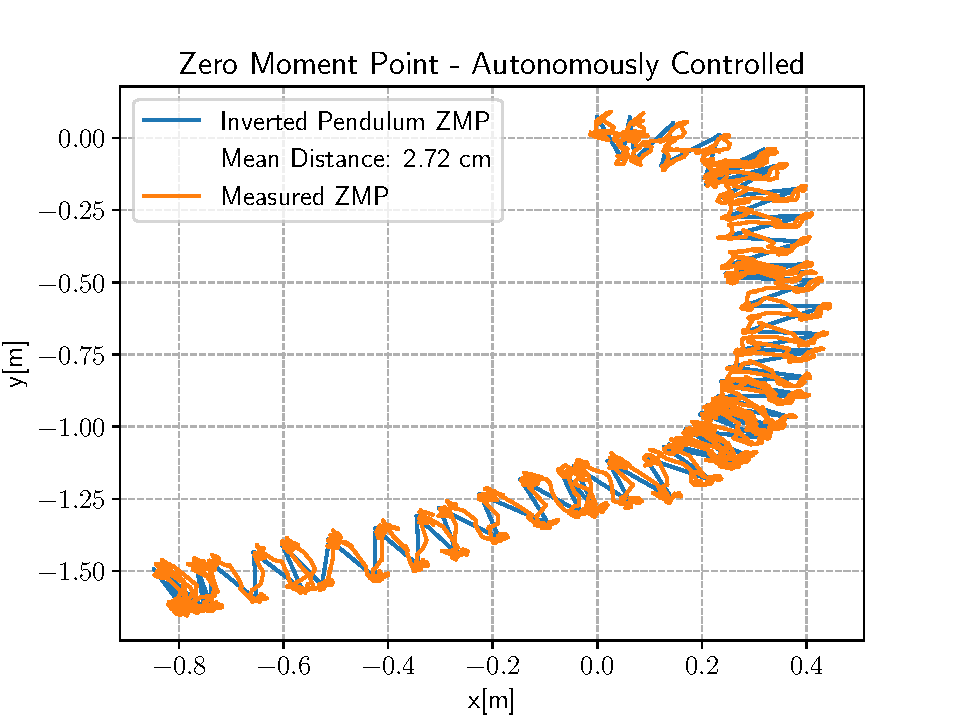
\includegraphics[scale=.35]{chapters/05_experiments/02_autonomous_walking/out_of_sight_walk_01_zmp.pdf}}
	\subcaptionbox{Environment Scanning - Behavior}%
	[.4\linewidth]{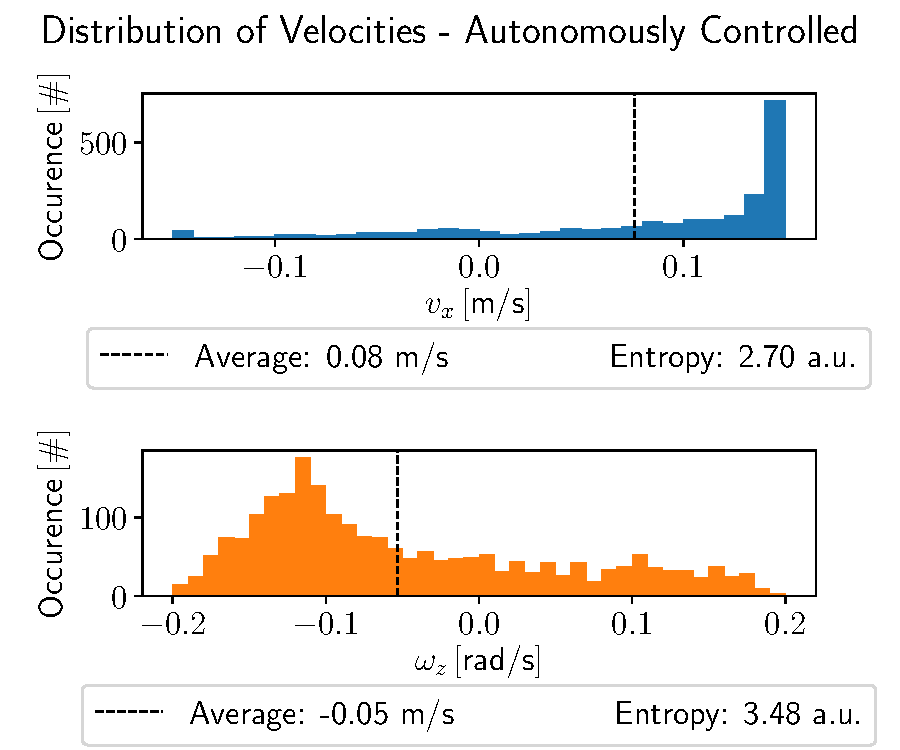
\includegraphics[scale=.35]{chapters/05_experiments/02_autonomous_walking/out_of_sight_walk_01_entropy.pdf}}
	\caption{}
	\label{fig::525_aw_basic}
\end{figure} 
\begin{figure}[h]
	\centering
	\subcaptionbox{Dynamic Environment}%
	[.4\linewidth]{\animategraphics[height=1.2in,loop,autoplay]{20}{chapters/05_experiments/02_autonomous_walking/dynamic_walk_01/frame-}{001}{031}}
	\subcaptionbox{Semantic Understanding}%
	[.4\linewidth]{\animategraphics[height=1.2in,loop,autoplay]{20}{chapters/05_experiments/02_autonomous_walking/semantic_walk_01/frame-}{001}{046}}
	\caption{}
\label{fig::525_aw_gif_additional}
\end{figure} 
\begin{figure}[h]
	\centering
	\subcaptionbox{Dynamic Environment - Dynamic Balance}%
	[.4\linewidth]{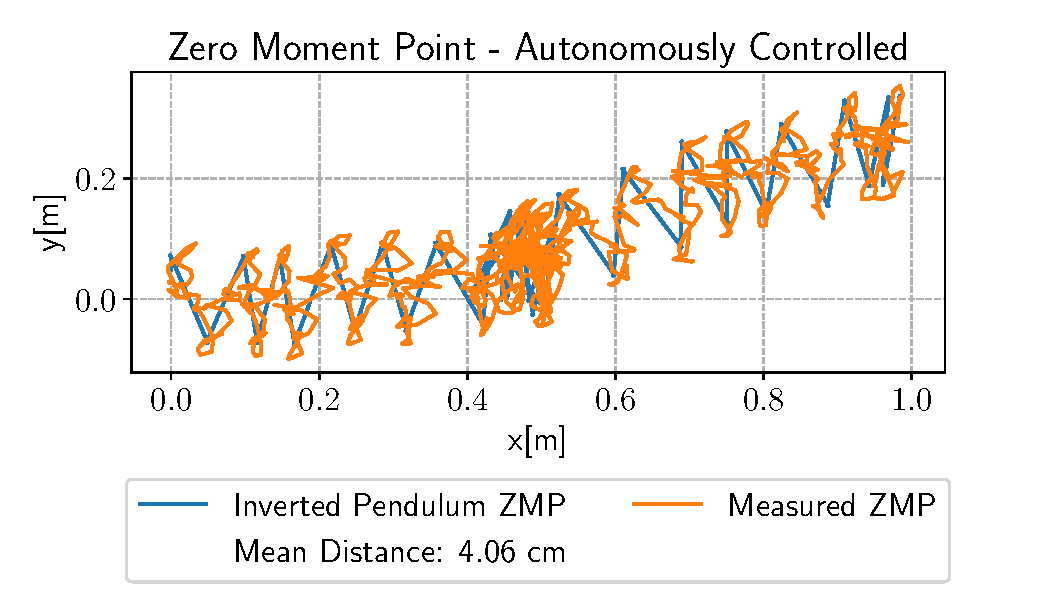
\includegraphics[scale=.35]{chapters/05_experiments/02_autonomous_walking/dynamic_walk_01_zmp.pdf}}
	\subcaptionbox{Dynamic Environment - Behavior}%
	[.4\linewidth]{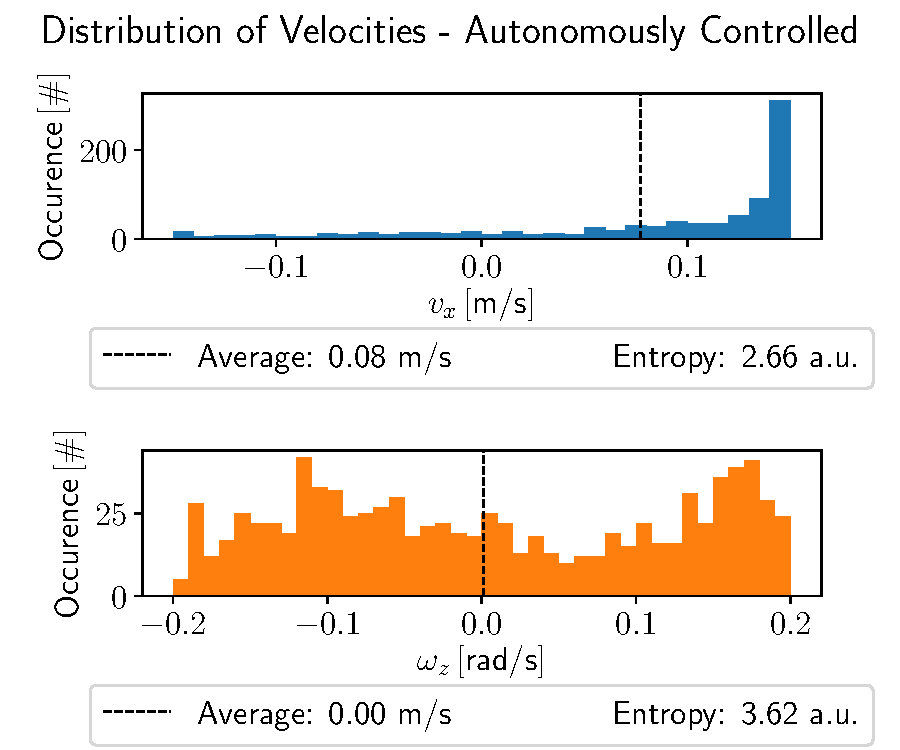
\includegraphics[scale=.35]{chapters/05_experiments/02_autonomous_walking/dynamic_walk_01_entropy.pdf}}
	\subcaptionbox{Semantic Understanding - Dynamic Balance}%
	[.4\linewidth]{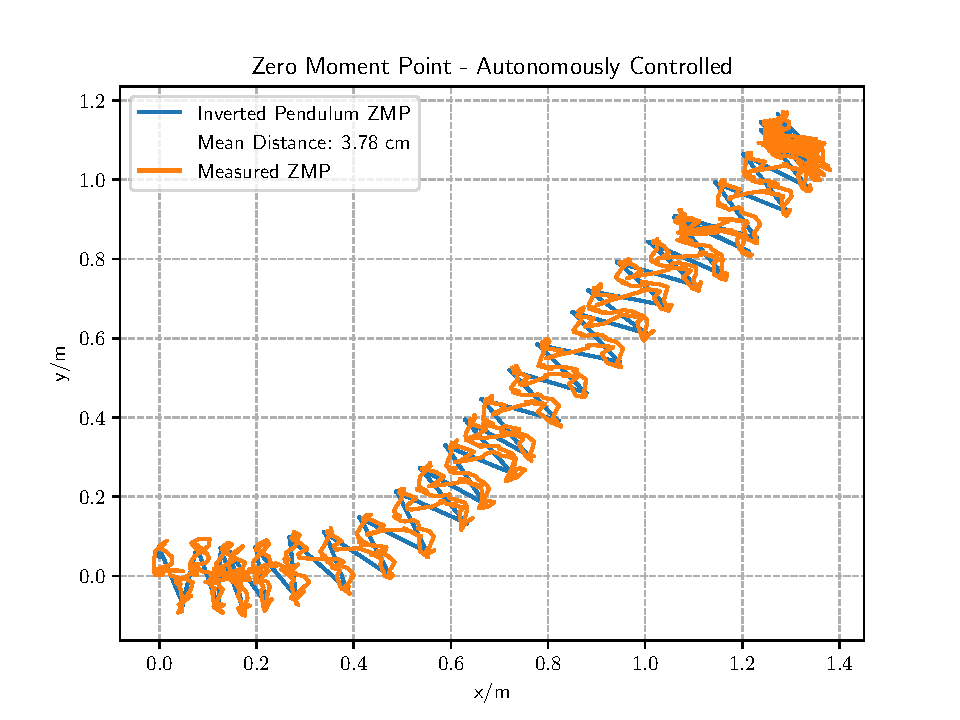
\includegraphics[scale=.35]{chapters/05_experiments/02_autonomous_walking/semantic_walk_01_zmp.pdf}}
	\subcaptionbox{Semantic Understanding - Behavior}%
	[.4\linewidth]{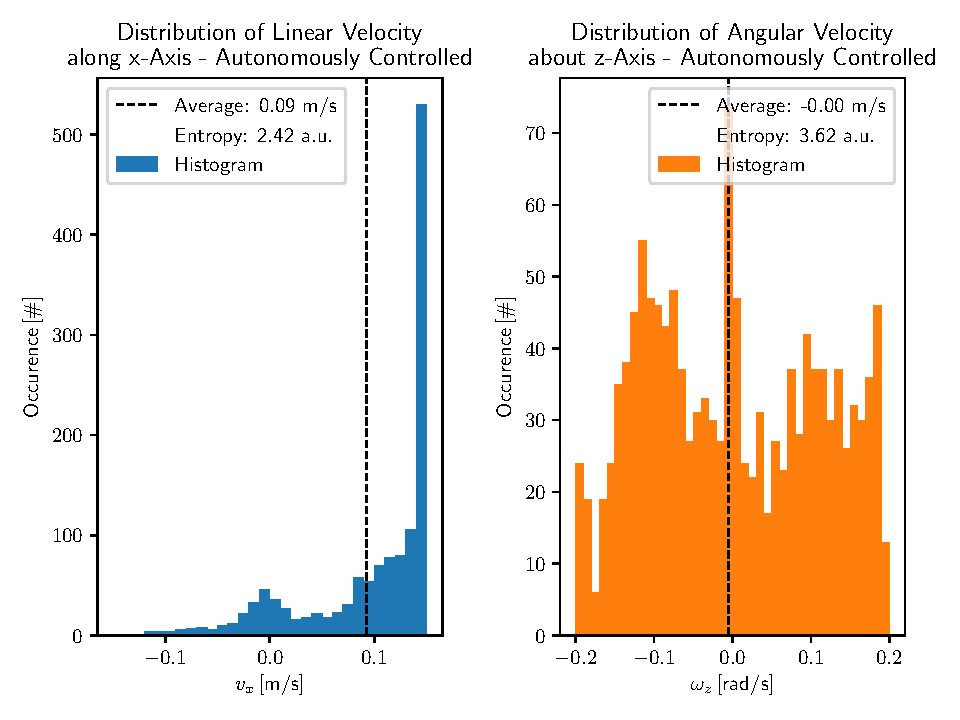
\includegraphics[scale=.35]{chapters/05_experiments/02_autonomous_walking/semantic_walk_01_entropy.pdf}}
	\caption{}
	\label{fig::525_aw_additional}
\end{figure}
\begin{figure}[h]
	\centering
	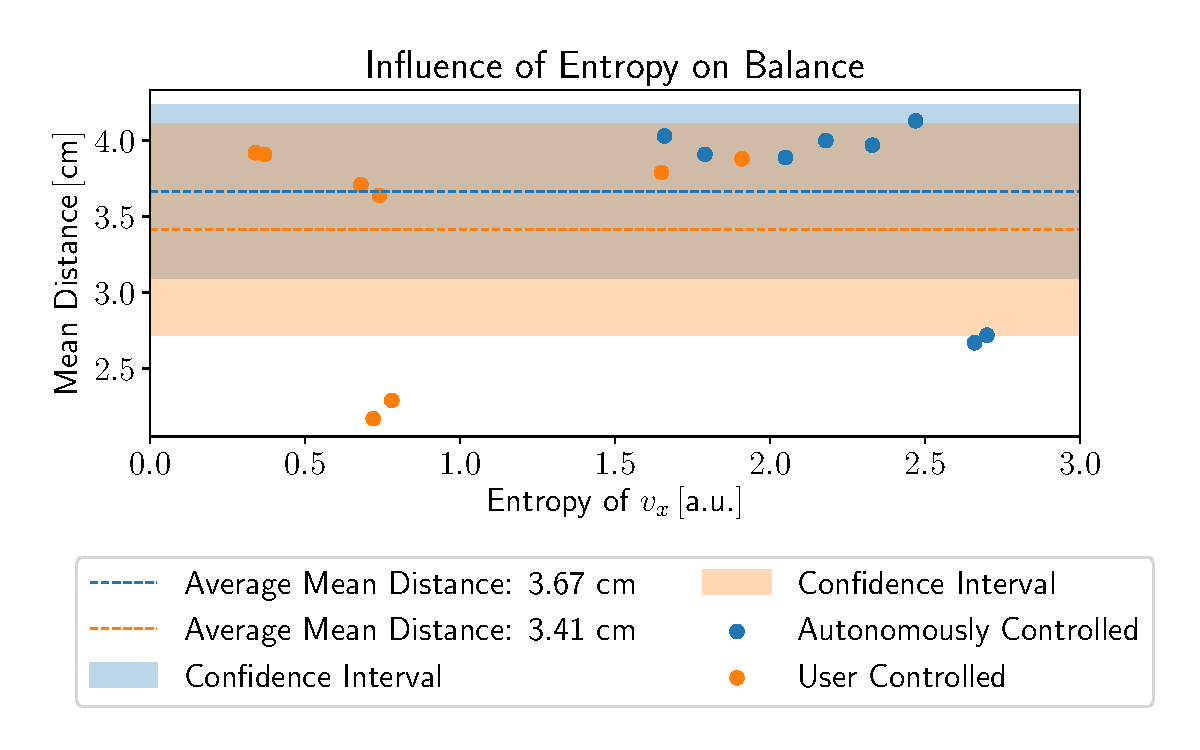
\includegraphics[scale=.6]{chapters/05_experiments/02_autonomous_walking/entropy_against_balance.pdf}
	\caption{meanaw 3.67, meanuc 3.41, stdaw 0.56, stduc 0.69}
	\label{fig::525_entropy_balance}
\end{figure}
\subsection{Proximal Policy Optimization}
